\documentclass[12pt]{article}
\usepackage[a4paper,top=1cm,bottom=2cm,left=1.5cm,right=1.5cm]{geometry}
\usepackage{framed}
\linespread{0.95}
\usepackage{graphicx} % Required for inserting images

\begin{document}
\title{\textbf{Progettazione Data warehouse (SCHEMA)}}
\author{\textit{Carlo Migliaccio}}
\date{Novembre 2023}
\maketitle

\section{Progettazione concettuale (Dimensional Fact Model)}
\begin{enumerate}
    \item Identificazione del \textbf{fatto} (o dei fatti) di interesse
        
        $\rightarrow$ misure (attenzione all'additività!)
    \item Identificazione delle \textbf{dimensioni di analisi}

    $\rightarrow$ definisce la granularità del fatto che spesso non è la stessa della fonte primaria di dati (OLTP ad esempio). Ad esempio: 
    
    Data singola (OLTP) $\rightarrow$ Mese (OLAP)
    \item \textbf{gerarchie} (verificare la relazione 1:n). Prestare attenzione a:
        \begin{itemize}
            \item \textit{archi multipli/attributi configurazione }(valore limite per la scelta: 10)
            \item \textit{gerarchia condivisa}, non sdoppiare gerarchie che potrebbero essere condivise
            \item \textit{punti di convergenza}
            \item \textit{opzionalità delle dimensioni, degli attributi}
        \end{itemize}

        
 \end{enumerate}

\begin{center}
    \centering
    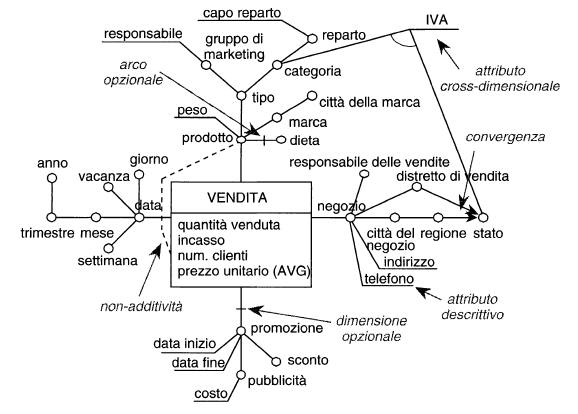
\includegraphics[width=0.8\linewidth]{dfm2.PNG}

    \textit{Esempio di DFM completo}
\end{center}

\section {Progettazione logica (Schema a stella)}

\begin{enumerate}
   
    \item Per ogni dimensione si crea una \texttt{tabella dimensionale} che contenga tutti gli attributi della gerarchia (qui si appiattiscono tutti i livelli di gerarchia), la chiave primaria è una \texttt{chiave surrogata} (autogenerata) che non ha nessun significato ai fini dell'analisi.

    Casi particolari: 
    \begin{itemize}
        \item \textsl{arco multiplo}:
        \begin{itemize}
            \item \textit{Tabella BRIDGE} (eventualmente con Peso: pensa alla percentuale di contributo nella scrittura di un libro); 
            \item \textit{push down} nella tabella dei fatti (da evitare)
            \item \textit{attributo configurazione}, se il dominio dell'attributo è limitato ad essere $\leq 10$
        \end{itemize}
        \item \textsl{dimensioni degeneri} (dimensioni con un solo attributo):
        \begin{itemize}
            \item \textit{tabella dimensionale} che abbia solo quell'attributo oltre la chiave surrogata;
            \item \textit{push down} nella tabella dei fatti $\rightarrow$ l'attributo entra a far parte della chiave primaria;
            \item \textit{junk dimension} che inglobi tutte le dimensioni degeneri (Attenzione alle cardinalità dei domini delle singole dimensioni degeneri, dal momento che la junk dimension contiene in modo combinatorio i valori delle dimensioni);
            \item \textit{soluzioni miste} che stiano a metà delle precedenti, ad esempio: alcune le metto nella tabella dei fatti mentre per altre posso scegliere un push down o una dimension table.
        \end{itemize}
    \end{itemize}

    

     \item Il fatto diventa la \texttt{tabella dei fatti} (centro stella), è quella che ha dimensione maggiore di tutto lo schema a stella. Lo schema della tabella dei fatti è costituito da:
    \begin{itemize}
        \item Le \textbf{chiavi delle dimensional table} che messe insieme costituiscono la chiave primaria;
        \item Le \textbf{misure} che diventano attributi.
    \end{itemize}
\end{enumerate}

\textbf{NOTE}:

\begin{itemize}
    \item le dimensioni di analisi condivise non vanno duplicate!
    \item è bene analizzare le query principali prima di congelare lo schema logico derivante da questa fase
    \item Gli attributi temporali sono da intendersi come: 
    \begin{itemize}
        \item Data $\Rightarrow$ GG/MM/AAAA
        \item Mese $\Rightarrow$ MM-AAAA
        \item Semestre $\Rightarrow$ S-AAAA, dove S è 1 o 2
    \end{itemize}
\end{itemize}

\begin{center}
    \centering
    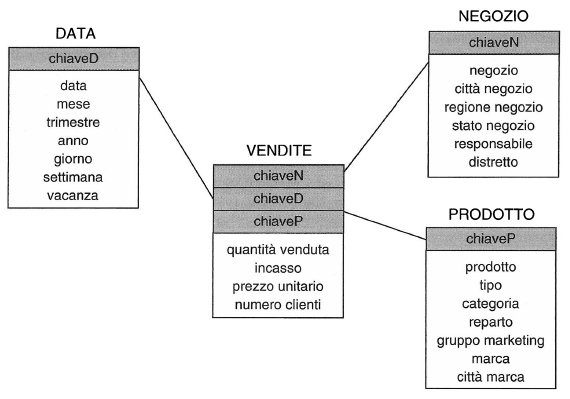
\includegraphics[width=0.6\linewidth]{star.PNG}
    
    \textit{Schema a stella}
\end{center}

\section{Query in SQL esteso}
\begin{enumerate}
    \item Analisi attributi nella clausola \texttt{SELECT}; 
    \item Costruzione del corpo della query con:
    \begin{itemize}
        \item  \texttt{FROM} $\Rightarrow$ scelta delle tabelle
        \item \texttt{WHERE} $\Rightarrow$ condizioni di join e predicati di selezione
        \item Attributi di \texttt{GROUP BY}. \textbf{Nota che...} se nelle \texttt{PARTITION BY} ci sono attributi non previsti nella \texttt{GROUP BY}, questi vi vanno inclusi, se non si può a causa di assenza di dipendenza funzionale del tipo A$\rightarrow$B (A determina B), c'è un problema di formulazione della query
        \item Funzioni aggregate nella \texttt{SELECT} 
    \end{itemize}
\end{enumerate}


\textbf{NOTA CHE...}
\begin{enumerate}
    \item L'operatore di \textbf{media aritmetica} è particolare: non sempre \texttt{AVG(Attributo)} produce un risultato che sia semanticamente corretto. 
    \textbf{Esempio} Se mi viene chiesto di calcolare una media giornaliera e nella partizione individuata dalla \texttt{GROUP BY} nonsono sicuro di avere una sola tupla per ogni giorno, allora AVG() non produce il risultato desiderato! Le soluzioni possibili a questo punto sono tre:
    \begin{enumerate}
        \item Applico la definizione di media aritmetica: \texttt{SUM(Attributo)/COUNT(DISTINCT Data)}
        \item uso una table function "customizzata" nella FROM
        \item uso \texttt{OVER} ricordandomi di mettere il \texttt{DISTINCT}
    \end{enumerate}
    \item Nelle \texttt{WINDOW} nel caso di calcolo di cumulativi, Top N, medie mobili e rank, l'\texttt{ORDER BY} è obbligatorio mentre non lo è per altri aggregati (es. somma);
    \item Le finestre di calcolo definite dopo la keyword \texttt{OVER} possono avere un'"apertura" più ampia rispetto a quella definita dalla \texttt{GROUP BY}. Si ricordi inoltre che nel caso di compresenza di OVER e GROUP BY, la OVER viene applicata al risultato della GB.
\end{enumerate}

\section{Viste materializzate}
\begin{quote}
    \texttt{CREATE MATERIALIZED VIEW NomeVista}

    \texttt{BUILD [IMMEDIATE | DEFERRED]}

    \texttt{REFRESH [COMPLETE | FAST] [ON COMMIT | ON DEMAND ]}

    \texttt{ENABLE QUERY REWRITE}

    \texttt{AS QueryVista}
\end{quote}

\begin{itemize}
    \item Osservare il \textbf{carico di lavoro (query)}, analizzando:
    \begin{itemize}
        \item \textsl{predicati di selezione}, non applico alla vista i predicati di selezione
        \item \textsl{attributi di Group By}
        \item \textsl{funzioni aggregate}
    \end{itemize}
    \item Determinare la vista che rappresenta il \textbf{denominatore comune}. Il fattore di riduzione deve essere almeno $\geq 10^3$, altrimenti non ha senso creare una vista materializzata
    \item Individuare correttamente la granularità della vista (attributo "meno profondo" in ogni gerarchia) $\Rightarrow$ rappresenta un vero e proprio \textbf{identificatore} della vista.
\end{itemize}

\subsection{Manutenzione di viste tramite TRIGGER}
Talvolta il prodotto DBMS che si utilizza potrebbe non avere a disposizione il comando \texttt{CREATE MATERIALIZED VIEW} e di conseguenza la gestione del build e refresh delle viste materializzate. In questo caso le viste diventano vere e proprie tabelle definite con l'istruzione \texttt{CREATE TABLE}, ma la loro gestione deve essere affidata alla presenza di uno o più \textbf{trigger} che ne gestiscano modifiche eventuali.

I trigger che tratteremo avranno sempre la stessa semantica e in particolare:
\begin{itemize}
    \item modo di esecuzione: \texttt{AFTER}. Il trigger viene eseguito appena \textbf{dopo} l'esecuzione dell'evento innescante (triggering event)
    \item granularità: \texttt{FOR EACH ROW}. Il trigger è eseguito una volta per ogni riga modificata dall'event innescante).
\end{itemize}
Gli altri due aspetti semantici possibili (BEFORE e FOR EACH STATEMENT) hanno alle spalle meccanismi spinosi che coinvolgono le proprietà ACID delle transazioni.


\textbf{Operazioni da svolgere: }
\begin{enumerate}
    \item Lettura dei valori degli attributi necessari dalle dimensioni
    \item Verifica esistenza tupla nella vista (nel caso di operazioni di tipo \texttt{INSERT})
    \item IF (tupla esiste) THEN ... \texttt{UPDATE} ELSE   \texttt{INSERT} 
\end{enumerate}

\subsubsection{Creazione di \texttt{MATERIALIZED VIEW LOG}}
Nel caso si scelga di scegliere per la vista materializzata un REFRESH di tipo FAST, c'è bisogno di creare prima della vista dei log materializzati che tengano traccia delle modifiche delle tabelle coinvolte dalla vista. Di seguito si riporta la sintassi di ORACLE:

\begin{quote}
    \texttt{CREATE MATERIALIZED VIEW LOG ON } Tabella

\texttt{WITH SEQUENCE, ROWID }

\texttt{(Id..., Campo1, Campo2, ..., CampoN)}

\texttt{INCLUDING NEW VALUES;}
\end{quote}

Lo schema di \textbf{Tabella} deve coinvolgere attributi che sono stati materializzati nella vista. 

\subsection{Note conclusive}
\begin{enumerate}
    \item Nella stesura del Trigger attenzione a non dimenticare la clausola \texttt{WHERE} nelle UPDATE, altrimenti si richia di modificare oltre alle tuple interessate anche quelle che prima erano a posto!
    \item Nella vista vanno memorizzate \textbf{funzioni aggregate distributive} (SUM,  COUNT, MIN, MAX) in modo che posso sempre ricostruire a livelli diversi di profondità altri operatori che distributivi non sono (es. AVG); 
    \item Normalmente, ad esclusione di situazioni particolari, non vanno messi predicati di selezione nella vista $\rightarrow$ la maggior parte delle volte questo può portare a perdita di generalità
\end{enumerate} 

\end{document}
